% Document class
% Document class
% chktex-file 44
% chktex-file 13
% chktex-file 8
\documentclass[12pt,a4paper]{article}%

% Packages
\usepackage[utf8]{inputenc}%
\usepackage[T1]{fontenc}%
\usepackage{indentfirst}%
\usepackage{geometry}%
\usepackage{setspace}%
\usepackage{times}%
\usepackage{lipsum}% For dummy text
\usepackage{graphicx}%
\usepackage{fancyhdr}%
\usepackage{titlesec}%
\usepackage{tocloft}%
\usepackage{amsmath,amssymb}%
\usepackage{caption}%
\usepackage{subcaption}%
\usepackage{booktabs}%
\usepackage{hyperref}%
\usepackage{natbib}%

% Geometry
\geometry{
  a4paper,
  left=3cm,
  right=2cm,
  top=2cm,
  bottom=2cm
}%

% Line spacing
\onehalfspacing%

% Page numbering
\pagestyle{fancy}%
\fancyhf{}%
\rfoot{\thepage}%

% Section formatting
\titleformat{\section}[block]{\normalfont\Large\bfseries}{\thesection}{1em}{}%
\titleformat{\subsection}[block]{\normalfont\large\bfseries}{\thesubsection}{1em}{}%

% Table of contents formatting
\renewcommand{\cftsecleader}{\cftdotfill{\cftdotsep}}%

% Paragraph formatting
\setlength{\parindent}{1.25em} % Indent for ALL paragraphs, including first
\setlength{\parskip}{0em}      % No extra spacing between paragraphs

\begin{document}

\begin{titlepage}
  \centering
  \vspace*{5cm}
  {\Huge \textbf{Modeling Household Carbon Footprints: Methods, Metrics, and Estimation Frameworks}}\\[2cm]
  {\large Master Thesis presented to the Department of Economics at the}\\
  {\large Rheinische Friedrich-Wilhelms-Universität Bonn}\\[1cm]
  {\large In Partial Fulfillment of the Requirements for the Degree of Master of Science (M.Sc.)}\\[2cm]
  Supervisor: [] \\[0.5cm]
  Submitted in [] by: \\[0.2cm]
  Anushka Mukherjee \\[0.2cm]
  Matriculation Number: 50075072
  \vfill
\end{titlepage}

% Table of Contents
\tableofcontents
\thispagestyle{empty}
\newpage

% Start of main text
\pagenumbering{arabic}
\setcounter{page}{1}


\section{Introduction}
\lipsum[1-2] % chktex 8

\section{Literature Review}
Climate change mitigation policies are heavily influenced by the development trajectories of nations and their respective stages of economic growth, as outlined in the fifth assessment report by the Intergovernmental Panel on Climate Change (IPCC, 2007). According to emission estimates for 2023 provided by the EDGAR database, global greenhouse gas (GHG) emissions increased by 1.9\% compared to 2022, reaching 53.0 Gt CO2eq. The major contributors to global GHG emissions in 2023 were China, the United States, India, the European Union (EU27), Russia, and Brazil, which together accounted for 62.7\% of the total global emissions. Carbon dioxide (CO2) produced by human activities remains the largest driver of global warming, with its concentration in the atmosphere having risen by 48\% above pre-industrial levels (before 1750) by 2020. The primary sources of CO2 emissions include the combustion of coal, oil, and natural gas, deforestation, livestock farming, the release of fluorinated gases from industrial equipment, and the use of nitrogen-based fertilizers (Weber \& Matthews, 2008). These activities have led to more frequent and severe weather events, including heatwaves and droughts, that are impacting regions around the world. In 2024, the United States experienced 27 weather and climate-related disaster events, each resulting in losses exceeding \$1 billion (NOAA, n.d.).

The growing acknowledgment of global warming as a significant threat has prompted international initiatives aimed at reducing greenhouse gas (GHG) emissions. These initiatives rely on accurate assessment and reporting of GHG emissions to inform climate policies (IPCC, 2007). Households account for 17\% of total global carbon dioxide (CO2) emissions, underscoring their critical role in addressing climate change. Understanding and mitigating residential contributions to greenhouse gas (GHG) emissions require prioritizing the household carbon footprint, a vital measure of emissions stemming from residential consumption (Du \& Zhong, 2024). Several methodologies are available for estimating GHG emissions, with the concept of carbon footprint gaining significant attention (Guinee, 2011). A carbon footprint is defined as the total GHG emissions caused directly and indirectly by an individual, organization, event, or product, traditionally calculated by summing emissions from every stage of a product or service's life cycle (Center for Sustainable Systems, 2024). Among the available methodologies, the GHG Protocol has emerged as a widely used framework for corporate GHG reporting, considering direct and indirect emissions resulting from household consumption. However, this method has limitations, such as double-counting and restricted adjustments for market dynamics (WBCSD, 2004). 


Another widely used approach is the Input-Output Analysis (IOA) method, a top-down model that calculates carbon footprints by analyzing monetary transactions between activities and extending them to an environmental level through greenhouse gas (GHG) emissions. This approach, known as Environmentally Extended Input-Output Analysis (EEIO), provides a macro-level view of the environmental impacts of economic activities (Encyclopedia of Ecology, 2019). For instance, a study using EEIO to examine the carbon footprints of Australian equity investments and Socially Responsible Investments (SRI) demonstrated that applying SRI criteria significantly reduces the carbon footprint of equity portfolios. This highlights equity investments as a major driver of economic activity and a crucial lever in advancing a sustainable economy (Chard, 2024).


Another frequently used method for calculating carbon emissions is the Emission Factor (EF) method. According to the Intergovernmental Panel on Climate Change (IPCC, 2019), the formula for estimating GHG emissions is:
\[
\text{GHG Emissions} = \text{Activity Data (AD)} \times \text{Emission Factor (EF)}
\]
Here, Activity Data (AD) refers to the scale of production or consumption activities that result in GHG emissions, such as fossil fuel use or electricity consumption. The Emission Factor (EF) represents the amount of GHG emitted per unit of activity, such as the emissions per liter of fuel burned or per kilowatt-hour of electricity consumed. Life Cycle Assessment (LCA) is a highly sophisticated tool for examining the environmental impact of products and services. It offers a holistic evaluation, tracing environmental consequences across every stage of a product's existence, from the extraction of raw materials to its final disposal—often described as a ``cradle-to-grave approach''. By analyzing phases such as production, distribution, usage, and end-of-life processes, LCA quantifies resource use, greenhouse gas emissions, and pollution affecting air, water, and soil systems (Global Climate Initiatives, 2023). A study leveraging LCA and household survey data provided precise calculations of carbon footprints by capturing emissions associated with daily consumption, household production activities, and the supply chain of consumed goods (Peng, 2021).

\vspace{5pt}

The model by Hakenes and Schliephake (2024) offers a fresh perspective on carbon footprint estimation by addressing the shortcomings of traditional static models. This consequentialist approach integrates market behaviors and industry-specific responses to provide a more dynamic and realistic analysis of household emissions. It highlights the connection between individual consumer decisions and broader emission outcomes, accounting for variables such as price elasticity and interdependencies between industries in both product and financial markets. By separating direct emissions tied to household activities from spillover effects influencing other sectors, this model delivers a more detailed and actionable understanding of household contributions to carbon emissions, paving the way for tailored climate strategies.


\section{Methodology}
\lipsum[3-4]

\section{The GHG Protocol}
The Greenhouse Gas (GHG) Protocol is a globally recognized standard for accounting and reporting greenhouse gas emissions. Developed in the late 1990s through a collaboration between the World Resources Institute (WRI) and the World Business Council for Sustainable Development (WBCSD), the GHG Protocol was officially launched in 2001 with the primary aim of providing a consistent and comprehensive framework for emissions accounting across corporate and public sectors. Over the years, its importance has grown significantly, with subsequent expansions such as the development of the GHG Protocol Scope 3 Standard in 2011, which broadened the accounting boundary to include indirect emissions across a company’s or household’s value chain. The historical motivation behind its creation was rooted in the need for greater transparency and comparability in emissions disclosures, especially as climate policy instruments and stakeholder expectations became increasingly sophisticated.

The principal reason for employing the GHG Protocol in household-level emissions analysis lies in its capacity to provide a standardized and granular approach to calculating emissions across different dimensions of behavior. It allows for a full inventory of climate impacts arising from everyday life—from fueling a car to investing in equity portfolios. Additionally, the protocol facilitates benchmarking across time and geography, making it possible to compare the carbon intensities of different households or regions. This is particularly valuable for policy-making, where a reliable basis for comparison is needed to design effective incentives, taxes, or subsidy programs aimed at reducing emissions. Moreover, with the rise of ESG (Environmental, Social, and Governance) investing, households are increasingly motivated to assess not only their consumption patterns but also the environmental implications of their financial choices. The GHG Protocol's inclusion of Scope 3 investment-related emissions is thus particularly timely and relevant.

The mathematical formulation under the GHG Protocol for calculating a household’s carbon footprint begins with the aggregation of emissions across three main scopes of emissions. The total carbon footprint of a household is expressed as:

\begin{equation}
CF_{\text{household}} = E_{\text{Scope 1}} + E_{\text{Scope 2}} + E_{\text{Scope 3}}
\end{equation}

Each of these components is calculated based on the product of activity data and corresponding emission factors. For Scope 1, this includes the quantity of fuel combusted in household-controlled devices or vehicles, multiplied by the fuel-specific emission factor. Scope 2 emissions are determined by multiplying electricity or district heating usage by grid-specific emission factors. Scope 3 is more complex and can be further disaggregated into emissions from the consumption of goods and services, and emissions from household investments. For the consumption subcategory, expenditures are multiplied by lifecycle emission factors derived from environmentally extended input-output models or product-level lifecycle assessments. For investment-based emissions, the monetary value of investments is multiplied by portfolio-weighted emission intensities of the respective industries.

Despite its widespread adoption, the traditional GHG Protocol approach has recognized limitations, particularly regarding its static nature and reliance on average emission factors. Recent literature emphasizes that more accurate household carbon footprint estimates require better representation of behavioral responses to price and policy signals. For example, Hertwich and Peters (2009) highlight that static inventories fail to capture the rebound effects and indirect market shifts that arise when households change consumption patterns in response to taxes or subsidies. Integrating behavioral elasticities into Scope 3 calculations would help address this gap by accounting for how consumers substitute goods or adjust spending in response to changing costs (Munksgaard et al., 2000). Additionally, several studies argue that using national average emission factors can mask significant regional differences. Lenzen et al. (2004) and Wiedmann (2009) both recommend refining emission estimates through regionally disaggregated electricity grid mixes, heating fuel profiles, and transport modes, as local supply chains often diverge substantially from national averages. By combining region-specific emission data with behavioral modelling, household carbon footprint accounting can better align with real-world dynamics and provide a stronger basis for targeted mitigation measures.

Moreover, the GHG Protocol framework can be further refined by incorporating time-series data, which would enable longitudinal comparisons and provide clearer insights into progress toward emissions reduction targets and the effectiveness of policy measures over time (Hertwich \& Peters, 2009). In addition, expanding the focus to include complementary sustainability metrics, such as water use, material intensity, and land footprint, would allow for a more comprehensive assessment of household environmental impacts beyond carbon alone (Wiedmann \& Minx, 2008). Taken together, these enhancements illustrate the evolving potential of the GHG Protocol to deliver a robust and nuanced picture of household sustainability.

To demonstrate how the GHG Protocol method can be applied in practice, the following section uses household consumption data from Spain for the year 2022 as an illustrative case. This example shows how direct, indirect energy, and value chain emissions are calculated within the three-scope framework and highlights the method’s practical use for identifying major sources of emissions.
Based on this calculation, the total household carbon footprint is estimated at approximately 11,828 kg CO$_2$e per year, with indirect emissions accounting for the largest share, which reflects a pattern widely documented in studies of household carbon footprints in high-income countries (Hertwich and Peters, 2009; Ivanova et al., 2016).

 Such insights can be pivotal for policy recommendations, such as encouraging low-carbon food choices, promoting public transport, or offering green investment options to households.

\subsection{Illustration: Application of the GHG Protocol to Spanish Household Consumption (2022)}

As an empirical demonstration, the GHG Protocol framework is applied to household expenditure data for Spain in 2022, illustrating how emissions are quantified and distributed across Scopes 1, 2, and 3 in practice. The data is sourced from the Spanish National Statistics Institute (INE), which reports average annual consumption expenditures per household disaggregated by COICOP classification. This dataset provides category-specific expenditure values and percentage structures, enabling assignment of appropriate emission factors to each type of consumption.

The total mean annual household expenditure is reported at €31,568. This amount is allocated across major consumption areas, including food and non-alcoholic beverages, housing and energy, transport, communication, and services such as restaurants and recreation. The corresponding structure percentages indicate the relative contribution of each category to total spending. For example, housing and energy account for approximately 32.4 percent of total expenditure, while food and beverages represent about 16.0 percent. Transport expenditures stand at 12.0 percent, with notable growth observed in service-related categories such as restaurants and hotels. A detailed breakdown of these categories is provided in Table 1 of the appendix.

Next, we calculate Scope 1 emissions. These emissions arise from the direct combustion of fossil fuels by households, primarily through private vehicle use and home heating. We use energy consumption data expressed in gigajoules (GJ) per capita and apply appropriate emission factors. According to Spain’s INE and international emission factor databases such as DEFRA and IPCC, petrol used for transport has an emission factor of 73.3 kg CO$_2$e/GJ, while natural gas used in heating has a slightly lower factor of 56.1 kg CO$_2$e/GJ.

% Ensure \usepackage{graphicx} is in your preamble

\begin{table}[h]
\centering
\caption*{\textbf{Table 4.1}: Direct Emissions from Household Energy and Transport (Scope 1)}\label{tab:scope1}
\resizebox{\textwidth}{!}{%
\begin{tabular}{lccc}
\toprule
\textbf{Energy Source} & \textbf{Consumption (GJ/hab)} & \textbf{Emission Factor (kg CO$_2$e/GJ)} & \textbf{Emissions (kg CO$_2$e)} \\
\midrule
Natural Gas (Transport) & 0.04 & 56.1 & 2.24 \\
Petrol (Transport)      & 14.44 & 73.3 & 1058.45 \\
Natural Gas (Heating)   & 0.73 & 56.1 & 40.95 \\
Petrol (Other)          & 0.18 & 73.3 & 13.19 \\
\midrule
\textbf{Total}          &       &       & \textbf{1114.83} \\
\bottomrule
\end{tabular}%
}
\end{table}


We then proceed to Scope 2 emissions, which pertain to purchased energy—namely electricity and district heating—used within the household but generated off-site. The average household in Spain consumed approximately 8.96 GJ of heating and cooling energy. The national grid's emission factor for such energy consumption, based on 2022 data, is estimated at 92.6 kg CO$_2$e per GJ.

\begin{table}[h]
\centering
\caption*{\textbf{Table 4.2:} Indirect Emissions from Heating and Cooling (Scope 2)}\label{tab:scope2}
\resizebox{\textwidth}{!}{%
\begin{tabular}{lccc}
\toprule
\textbf{Energy Source} & \textbf{Consumption (GJ/hab)} & \textbf{Emission Factor (kg CO$_2$e/GJ)} & \textbf{Emissions (kg CO$_2$e)} \\
\midrule
Heating/Cooling Energy & 8.96 & 92.6 & 829.70 \\
\midrule
\textbf{Total} & & & \textbf{829.70} \\
\bottomrule
\end{tabular}%
}
\end{table}

The most complex and voluminous part of the analysis involves Scope 3 emissions. These emissions arise from the indirect impacts of household consumption decisions, including the carbon embedded in food, manufactured goods, services, and transportation infrastructure. Each expenditure category is multiplied by a category-specific emission factor derived from lifecycle assessment databases. For example, the food category carries an emission factor of 0.50 kg CO$_2$e per euro spent, reflecting emissions from agriculture, processing, and distribution. Clothing, by contrast, has a lower factor of 0.25 kg CO$_2$e/€, while restaurant services, due to their energy intensity, have a higher factor of 0.40 kg CO$_2$e/€.

% Make sure you have \usepackage{booktabs} and \usepackage{graphicx} in your preamble

\begin{table}[h]
\centering
\caption*{\textbf{Table 4.3:} Consumption-Based Emissions (Scope 3)}\label{tab:scope3}
\resizebox{\textwidth}{!}{%
\begin{tabular}{lccc}
\toprule
\textbf{Category} & \textbf{Expenditure (€)} & \textbf{Emission Factor (kg CO$_2$e/€)} & \textbf{Emissions (kg CO$_2$e)} \\
\midrule
Food and non-alcoholic beverages & 5,050 & 0.50 & 2,525.00 \\
Alcoholic beverages and tobacco  &   481 & 0.30 &   144.30 \\
Clothing and footwear            & 1,232 & 0.25 &   308.00 \\
Housing and utilities            &10,243 & 0.25 & 2,560.75 \\
Furnishings                      & 1,296 & 0.30 &   388.80 \\
Health                           & 1,228 & 0.20 &   245.60 \\
Transport services               & 3,794 & 0.30 & 1,138.20 \\
Communications                   &   925 & 0.15 &   138.75 \\
Recreation                       & 1,534 & 0.35 &   536.90 \\
Education                        &   468 & 0.10 &    46.80 \\
Restaurants and hotels           & 2,953 & 0.40 & 1,181.20 \\
Miscellaneous goods and services & 2,364 & 0.30 &   709.20 \\
\midrule
\textbf{Total}                   &        &       & \textbf{9,883.55} \\
\bottomrule
\end{tabular}%
}
\end{table}

Finally, by summing the results from all three scopes, we obtain the total household carbon footprint for a typical Spanish household in 2022. The emissions distribution clearly reveals that Scope 3 emissions dominate, comprising nearly 84\% of the total. This insight aligns with broader research indicating that in high-income settings, the indirect emissions associated with consumption patterns far exceed direct household emissions.

% Make sure \usepackage{booktabs} is in your preamble

\begin{table}[h]
\centering
\caption*{\textbf{Table 4.4:} Total Household Carbon Footprint by Scope}\label{tab:total_emissions}
\begin{tabular}{lc}
\toprule
\textbf{Scope} & \textbf{Emissions (kg CO$_2$e)} \\
\midrule
Scope 1 & 1,114.83 \\
Scope 2 &   829.70 \\
Scope 3 & 9,883.55 \\
\midrule
\textbf{Total} & \textbf{11,828.08} \\
\bottomrule
\end{tabular}
\end{table}


This empirical illustration not only validates the functionality of the GHG Protocol when applied to real-world household data but also emphasizes the critical role of consumption behavior in shaping emissions outcomes. The findings suggest that while improvements in home energy efficiency and cleaner fuels are valuable, the most substantial reductions may be achieved through systemic shifts in consumption patterns, such as transitioning to plant-based diets, reducing air travel, or shifting investments away from carbon-intensive industries.
\section{Life Cycle Assessment (LCA) Method}
The LCA method calculates emissions throughout the entire life cycle of a product or service, from production to disposal. This model captures emissions from every stage of the supply chain and provides a comprehensive assessment of indirect emissions.

The carbon footprint for a single industry using the LCA approach is:
\begin{equation}
   fp_h = q_h \cdot \text{LCA}_j 
\end{equation}

where \(q_h\) is the quantity consumed by household \(h\), and \(\text{LCA}_j\) represents the life cycle emissions per unit in industry \(j\).


\subsection{Methodology for Household Carbon Footprint Calculation based on LCA approach}
This section adapts the framework developed by Peng et al. (2021) to estimate household carbon footprints by combining complementary life cycle assessment (LCA) techniques. Aligned with principles outlined in Guinée (2011) and comparative reviews such as Matthews et al. (2008) and Steubing et al. (2022), the approach quantifies both direct and embodied greenhouse gas (GHG) emissions, together with net carbon sequestration linked to household-level activities.

The methodology integrates three LCA variants to address the system boundary limitations inherent in partial assessments: (1) Process-based LCA is applied to quantify emissions from agricultural operations and livestock production, capturing emissions embedded in material inputs and field-level activities; (2) Input–Output LCA extends the boundary to indirect emissions embedded in household consumption of energy, food, housing, and transport, using environmentally extended input–output (EEIO) tables (Weber and Matthews, 2008); (3) Hybrid LCA bridges both levels by combining process inventory detail with macroeconomic input–output linkages, reducing truncation errors and capturing carbon flows related to afforestation, durable goods, and other land-use changes (Crawford et al., 2018; Shen et al., 2023).

Following Peng et al. (2021), the model distinguishes five core domains: direct energy use, short-lived and durable consumption, household agriculture, afforestation, and livestock management. Activity-specific emissions are parameterized using survey-derived data and regionally adjusted emission factors in accordance with IPCC (2019) guidelines. This combined accounting framework quantifies net household carbon flows as the balance of annual GHG emissions and sequestration within a unified system boundary:

\begin{equation}
CF_i = \sum_{n} E_{in} + \sum_{m} S_{im}
\end{equation}
where $CF_i$ represents the Carbon footprint of household $i$, $E_{in}$ is the annual carbon emissions of household $i$ in category $n$ and $S_{im}$ is the annual carbon sequestration of household $i$ in category $m$. This disaggregated yet integrated structure provides the basis for the following activity-specific equations, which formally express how annual household emissions and sequestration are calculated within each functional domain.

\subsection{Carbon Emissions from Direct Energy Consumption}
The emissions from household direct energy use are estimated by multiplying the quantity of fuel consumed by its corresponding emission factor. For each household ii, the total emissions attributable to direct fuel combustion are calculated as:
\begin{equation}
E_{id} = \sum_d (F_{id} \cdot EF_d)
\end{equation}
where $F_{id}$ denotes the annual consumption of household $i$  for fuel type $d$. The fuel-specific emission factor $E_{id}$ combines oxidation efficiency, fuel composition, and calorific value, consistent with IPCC (2019) guidelines:
\begin{equation}
EF_d = OX_d \cdot \left(C_{o,d} \cdot \frac{12}{44} + C_{h,d} \cdot \frac{12}{16}\right) \cdot H_d \cdot 10^{-9}
\end{equation}
Here, $OX_d$ represents the oxidation efficiency, typically assumed to be 100\% for complete combustion; $C_{o,d}$ and $C_{h,d}$ are the fuel-specific emission coefficients for CO$_2$ and CH$_4$, respectively; and $H_d$ denotes the net calorific value of the fuel. The conversion factors ensure that carbon content is expressed in consistent units of tonnes CO$_2$ equivalent per unit of fuel input.

\subsection{Carbon Emissions from Living Consumption}

Emissions attributable to household consumption of goods and services are divided into two categories: short-lived products and durable consumer goods. The total annual emissions from short-lived consumption are given by:

\begin{equation}
E_{if} = \sum_f (EF_f \cdot C_{if})
\end{equation}

where $E_{if}$ denotes the annual carbon emissions from short-lived good $f$, $C_{if}$ is the quantity of product $f$ consumed by household $i$, and $EF_f$ is its corresponding life cycle emission factor. For durable consumer products, the embodied emissions are amortized over the product's expected service life to obtain an annualized footprint:

\begin{equation}
E_{ij} = \sum_j \frac{(EF_j \cdot C_{ij})}{L_j}
\end{equation}

Here, $E_{ij}$ represents the annual emissions associated with durable product $j$, $C_{ij}$ is the total quantity purchased, $EF_j$ is the relevant life cycle emission factor, and $L_j$ is the product’s average lifetime (in years). This treatment ensures that emissions embedded in capital household goods are allocated proportionally across their period of use, consistent with standard LCA accounting conventions.


\subsection{Carbon Footprint in Agricultural Activities}

Emissions and sequestration associated with household-level agricultural production are accounted for through inputs, on-site operations, and net biomass growth. The total annual carbon footprint from agricultural activities for household $i$ is calculated as:

\begin{equation}
CF_{ia} = \sum_a (EF_a \cdot M_{ia}) + \sum_t (EF_t \cdot FS_{ia}) + \sum_v (B_v \cdot 0.475)
\end{equation}

Here, $CF_{ia}$ denotes the net carbon impact of agricultural activities. $M_{ia}$ represents the quantity of material input $a$ (such as fertilizers or pesticides) applied by household $i$, with an associated emission factor $EF_a$. The second term accounts for emissions from field operations, where $FS_{ia}$ is the cultivated field size and $EF_t$ is the emission factor per unit area for operation $t$ (e.g., tillage, irrigation). The final term reflects the carbon sequestered in above-ground biomass, with $B_v$ indicating the dry biomass yield for crop or vegetation type $v$, multiplied by a standard carbon content coefficient of 47.5\% (IPCC default for plant biomass).


\subsection{Carbon Sequestration from Afforestation}

Carbon sequestration through household-level afforestation is estimated based on the area of land dedicated to tree planting and the average carbon stock of the tree species established. The annual sequestration from afforestation for household $i$ is given by:

\begin{equation}
S_{iaf} = FS_{iaf} \cdot CS_{\text{citrus}}
\end{equation}

In this expression, $S_{iaf}$ represents the amount of carbon sequestered through afforestation activities, $FS_{iaf}$ denotes the field size (in hectares) allocated for tree planting by household $i$, and $CS_{\text{citrus}}$ is the mean carbon stock per unit area for citrus trees or other comparable species. The carbon stock factor reflects the average annual carbon uptake, accounting for biomass accumulation under local growth conditions.


\subsection{Carbon Emissions from Livestock Raising}

Emissions from household livestock activities include fodder production, enteric fermentation, and manure management. The total annual emissions from livestock raising for household $i$ are calculated as:

\begin{equation}
E_{il} = \sum_f (EF_{if} \cdot F_{if}) + \sum_l (EF_{il} \cdot N_{il})
\end{equation}

In this formulation, $E_{il}$ represents the total carbon emissions attributable to livestock-related activities. $F_{if}$ denotes the annual quantity of fodder consumed by livestock, multiplied by the corresponding emission factor $EF_{if}$ to account for upstream impacts of fodder cultivation and transport. The second term captures direct emissions from livestock, where $N_{il}$ is the number of animals of type $l$ and $EF_{il}$ is the per-animal emission factor, which includes methane emissions from enteric fermentation and nitrous oxide from manure management.



\subsection{Aggregate Formula for Household Carbon Footprint}

The total household carbon footprint ($CF_{\text{total}}$) aggregates emissions and sequestration from direct energy use, living consumption, agricultural production, afforestation, and livestock raising, as specified in Equations (4) to (10).

\begin{align}
CF_{\text{total}} = & \underbrace{\sum_d \left(F_{id} \cdot EF_d\right)}_{\text{Direct energy}} + 
\underbrace{\sum_f \left(EF_f \cdot C_{if}\right) + \sum_j \frac{\left(EF_j \cdot C_{ij}\right)}{L_j}}_{\text{Living consumption}} \nonumber \\
& + \underbrace{\sum_a \left(EF_a \cdot M_{ia}\right) + \sum_t \left(EF_t \cdot FS_{ia}\right) + \sum_v \left(B_v \cdot 0.475\right)}_{\text{Agriculture}} \nonumber \\
& - \underbrace{\sum_{iaf} \left(FS_{iaf} \cdot CS_{\text{citrus}}\right)}_{\text{Afforestation}} +
\underbrace{\sum_f \left(EF_{if} \cdot F_{if}\right) + \sum_l \left(EF_{il} \cdot N_{il}\right)}_{\text{Livestock}}.
\label{eq:aggregate}
\end{align}

By integrating disaggregated activity data with region-specific emission factors, this aggregate formulation is a consistent representation of the net annual GHG balance at the household level, consistent with best practices in household carbon accounting (Ivanova et al., 2016; Dubois et al., 2019). 

Beyond its measurement function, this structure highlights how household decisions on energy use, consumption patterns, and land management jointly influence emissions outcomes (Hertwich and Peters, 2009). Such clarity enables scenario analysis of behavioral shifts and technological choices, informing targeted interventions like carbon price adjustments, renewable energy adoption incentives, or compensation for sequestration through land-based measures (Rogelj et al., 2018; Steubing et al., 2022). As shown in recent household-level studies, aligning micro-level incentives with broader climate objectives is essential to internalize externalities and realize cost-effective emission reductions (Wiedmann et al., 2020).

\subsection{Household Emissions Breakdown under LCA}

An integrated life cycle assessment (LCA) illustration clarifies how the total household carbon footprint, as defined by Equations (4) to (10), is distributed across major activity domains. Drawing on estimates from Peng et al.\ (2021), Sala et al.\ (2014), and Matthews et al.\ (2008), direct household energy use, including heating fuels and private vehicle fuels, accounts for approximately 20\% to 30\% of total greenhouse gas emissions. Living consumption, which covers short-lived goods, food purchases, and services, represents the largest share at about 50\% to 60\%. This highlights the significant upstream emissions embodied in supply chains. Within this category, food-related impacts illustrate the importance of production and distribution processes rather than any single consumption choice. For instance, staples such as cereals, fruits, and vegetables generally have lower average emission intensities than more resource-intensive foods, but all contribute to the overall footprint. Durable goods, including household appliances and furniture, add an additional 5\% to 10\% of total emissions when annualized, showing the relevance of product lifespan and embedded material flows. 

Together, this evidence shows that focusing only on direct household fuel use underestimates the total climate impact of residential lifestyles because indirect emissions embedded in goods and services account for most impacts, as discussed by Hertwich and Peters (2009). A comprehensive, activity-based LCA offers a more realistic basis for identifying mitigation options such as improving building energy performance, extending product lifespans, sourcing materials more sustainably, and investing in land-based carbon sequestration. This broader perspective supports the development of household-level strategies that address systemic drivers of emissions rather than isolating individual consumption categories.


\begin{figure}[h]
\centering
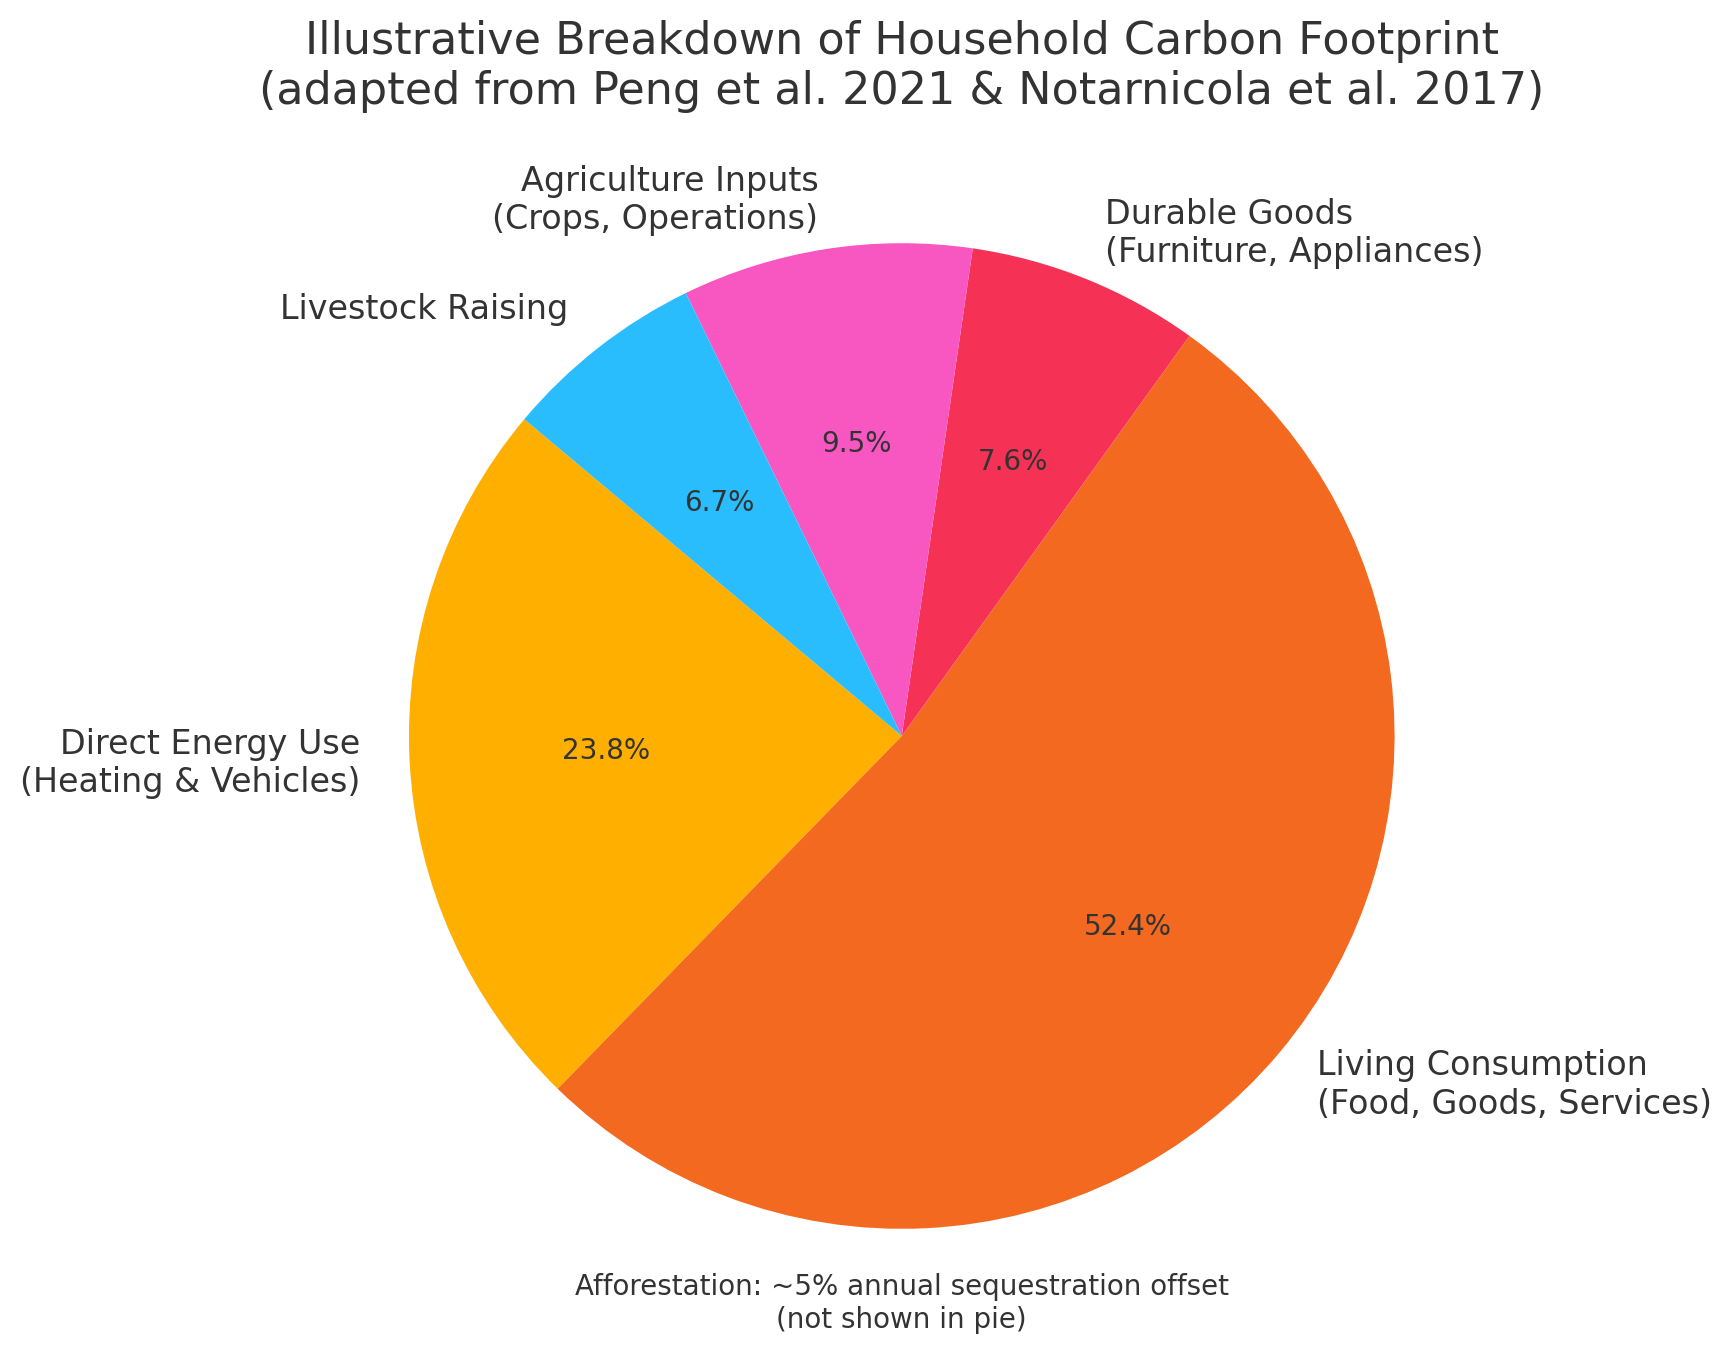
\includegraphics[width=0.8\linewidth]{LCA_pie.png}
\caption{Relative contributions of household activities to carbon footprints}
\end{figure}

\section{Input–Output Model and Carbon Footprint Estimation}
The environmentally extended Input-Output (EEIO) framework provides a macroeconomic approach for quantifying household carbon footprints by tracing both direct and upstream greenhouse gas (GHG) emissions embedded in goods and services. 

\subsection{Leontief Input–Output Framework}

We begin with the standard Leontief system, where total output \( \mathbf{X} \) is the sum of intermediate input requirements and final demand:

\begin{equation}
\mathbf{X} = \mathbf{A} \mathbf{X} + \mathbf{F}.
\end{equation}

Solving for total output yields the fundamental input–output identity:

\begin{equation}
\mathbf{X} = (\mathbf{I} - \mathbf{A})^{-1} \mathbf{F}.
\end{equation}

Here, \( \mathbf{A} \) is the technical coefficient matrix, \( \mathbf{F} \) is the vector of household final demand, and \( (\mathbf{I} - \mathbf{A})^{-1} \) is the Leontief inverse, which accounts for the total production required (both direct and indirect) to satisfy final demand.

\subsection{Technical Coefficient Matrix}

Each element \( A_{ij} \) of the matrix \( \mathbf{A} \) is defined as:

\begin{equation}
A_{ij} = \frac{z_{ij}}{x_j},
\end{equation}

where \( z_{ij} \) denotes the monetary value of inputs from sector \( i \) to sector \( j \), and \( x_j \) is the total output of sector \( j \). The matrix \( \mathbf{A} \) reflects the technological input structure of the economy.

\subsection{Stability of the Leontief Inverse}

The Leontief inverse \( (\mathbf{I} - \mathbf{A})^{-1} \) exists and is finite if the matrix \( \mathbf{A} \) satisfies the stability condition \( \rho(\mathbf{A}) < 1 \), where \( \rho(\cdot) \) denotes the spectral radius (i.e., the largest absolute eigenvalue). This condition ensures that the production system is productive and does not require infinite inputs. In applied input--output tables, a sufficient (but not necessary) condition is that the column sums of \( \mathbf{A} \) are each less than one:
\[
\sum_i A_{ij} < 1 \quad \text{for all } j.
\]
This implies that each sector uses less than one unit of intermediate input to produce one unit of output, a condition that is generally satisfied in empirical datasets (Miller and Blair, 2009).

\subsection{Carbon Footprint Estimation via Input–Output Modelling}

The environmentally extended input–output (EEIO) model estimates household carbon footprints by applying sectoral emission intensities to the total output vector required to satisfy final demand:

\begin{equation}
\mathbf{E} = \mathbf{C} (\mathbf{I} - \mathbf{A})^{-1} \mathbf{F},
\end{equation}

where \( \mathbf{C} \) is the vector of direct emission intensities (e.g., kg CO\textsubscript{2}e per euro of output), and \( \mathbf{E} \) is the resulting emissions attributable to household consumption. This formulation captures both direct and upstream (supply chain) emissions associated with consumption.

\subsection{Tiered Decomposition of Household Emissions}

Following Matthews et al.~(2008) and Long et al.~(2019), the total household footprint can be analytically decomposed into three tiers:

\paragraph{Tier 1: Direct Emissions}

\begin{equation}
\mathbf{E}_1 = \mathbf{C}_d \cdot \mathbf{F}_d,
\end{equation}

where \( \mathbf{F}_d \) is household consumption of directly combusted fuels and \( \mathbf{C}_d \) is the corresponding emission intensity vector.

\paragraph{Tier 2: Indirect Energy Emissions}

\begin{equation}
\mathbf{E}_2 = \mathbf{C}_e \cdot (\mathbf{I} - \mathbf{A})^{-1} \cdot \mathbf{F}_e,
\end{equation}

with \( \mathbf{F}_e \) representing consumption of electricity and district heating, and \( \mathbf{C}_e \) their emission intensities.

\paragraph{Tier 3: Indirect Supply Chain Emissions}

\begin{equation}
\mathbf{E}_3 = \mathbf{C} \cdot \left[(\mathbf{I} - \mathbf{M})(\mathbf{I} - \mathbf{A})\right]^{-1} \cdot \left[(\mathbf{I} - \mathbf{M}) \cdot \mathbf{F} + \mathbf{EX} \right],
\end{equation}

where \( \mathbf{M} \) is a diagonal matrix of sectoral import shares, and \( \mathbf{EX} \) accounts for exports. This import-adjusted EEIO formulation ensures emissions are assigned to domestic demand (Long et al., 2019; Sheng et al., 2024).

\paragraph{Total Household Footprint.}  
Combining all tiers, the household footprint is:

\begin{equation}
    \mathbf{E}_{\text{total}} = \mathbf{E}_1 + \mathbf{E}_2 + \mathbf{E}_3.
\end{equation}

This integrated EEIO framework mitigates truncation and boundary errors typical of process-based LCA, capturing the full feedback loops of modern economies (Matthews et al., 2008; Steubing et al., 2022).


\subsection{Illustrative Application of the Input-Output Model}

In this illustration, pre-calculated environmentally extended emission intensities (kg CO$_{2}$e per euro spent) are applied to household consumption data for France, Spain, and Germany for 2021. These intensities represent the aggregated effect of $\mathbf{C} {(\mathbf{I}-\mathbf{A})}^{-1}$ and are derived from the EXIOBASE multi-regional input-output (MRIO) model, as accessed via Climatiq.io. The method aligns with the tier-3 comprehensive accounting approach discussed in Matthews et al.~(2008), Long et al.~(2019), and Sheng et al.~(2024).

\subsection{Data and Methodology}

The Leontief inverse $(\mathbf{I} - \mathbf{A})^{-1}$ then expands final demand to include both direct and indirect production requirements.

\[
EF_i = \sum_{j} C_j L_{ji}, 
\quad \text{where} \quad 
L = {(\mathbf{I} - \mathbf{A})}^{-1}.
\]

Here, $C_j$ denotes the direct emissions intensity for producing sector $j$, and $L_{ji}$ represents the total requirements linking producing sectors $j$ and $i$. The resulting spend-based factors are published through Climatiq.io, which provides up-to-date coefficients aggregated from EXIOBASE under a permissive data license \citep{EXIOBASEsource}.

To ensure numerical stability, EXIOBASE balances its input-output tables using harmonised supply-use statistics, preventing divergence in the Leontief inverse. An additional feasibility check confirms that the sum of each column in $\mathbf{A}$ remains below unity, preserving the productive structure required for invertibility.

Annual household final consumption expenditure for France, Spain, and Germany was sourced from Eurostat for the year 2021 and harmonised to euros at the average annual exchange rate. For each expenditure category $i$ and country $c$, the household carbon footprint is estimated by multiplying the national expenditure by the corresponding spend-based factor:

\[
E_{i,c} = F_{i,c} \times EF_i.
\]

For instance, for France, the estimated annual household spending on food and non-alcoholic beverages is approximately

\[
F_{\text{food,FR}} = 1.322 \times 10^9 \times 0.139 = 183.8 \times 10^9~\text{EUR}.
\]

Multiplying this by the category-specific factor of 0.48~kg CO$_2$e per euro yields an estimated

\[
E_{\text{food,FR}} = 183.8 \times 10^9 \times 0.48 = 88.2 \times 10^6~\text{tonnes CO}_2\text{e}.
\]

The same procedure is applied across all final demand categories and for Spain and Germany. This method follows the tier-3 EEIO approach and systematically allocates upstream supply chain emissions, providing a comprehensive perspective on the consumption-driven climate impact of households. All emission factors are listed in Appendix~A, Table~2.

\subsection{Results}

The resulting household carbon footprints for 2021 are summarized in Tables~3--5 in Appendix~A. The total estimated footprints are approximately 420~Mt~CO$_2$e for France, 227~Mt~CO$_2$e for Spain, and 546~Mt~CO$_2$e for Germany.

Housing, food, and transport account for the largest shares of total household emissions in all three countries. These estimates demonstrate how the environmentally extended input-output (EEIO) approach captures indirect supply chain emissions embedded in upstream production, which are excluded from territorial greenhouse gas (GHG) inventories that measure only direct domestic emissions.

Unlike conventional GHG inventories or product-level life cycle assessments (LCA) that typically track physical quantities of fuel or goods consumed, the EEIO method allocates emissions based on household expenditure across all final demand categories. This spend-based framework enables the tracing of embodied emissions in goods and services, including imported products, providing a more complete perspective on consumption-driven impacts.

The scale and sectoral structure of the results are consistent with earlier multi-regional input-output analyses for Europe (e.g., Matthews et al.~2008; Sheng et al.~2024), which report housing energy use, food supply chains, and private mobility as the dominant drivers of household footprints. The method is widely applied due to its ability to integrate complex supply chain interactions and incorporate international trade adjustments (Long et al.~2019). This confirms that the IO model, when combined with up-to-date household expenditure data, remains an effective tool for quantifying the full indirect climate impact of household demand.


\subsection{Comparative Assessment of LCA and EEIOA for Household Carbon Footprint Estimation}

Life cycle assessment (LCA) and environmentally extended input--output analysis (EEIOA) are both established approaches for estimating household carbon footprints but differ in system boundaries and detail. LCA quantifies emissions by summing process-based impacts across all life cycle stages, often including capital goods and infrastructure explicitly.

In this illustration, the household carbon footprint is quantified using an LCA framework adapted from Steubing et al.~(2022). The structure of the total footprint, previously defined in Equation~(11), can be re-stated as:

\begin{equation}
\text{CF}_{\text{total}} = \sum_d (F_{id} \cdot EF_d) 
+ \sum_f (C_{if} \cdot EF_f) 
+ \sum_j \left( \frac{C_{ij} \cdot EF_j}{L_j} \right)
+ \sum_a (M_{ia} \cdot EF_a)
- \sum_t (S_{it} \cdot CS_t).
\end{equation}
where fuel use, short-lived and durable goods, capital goods lifespan, material inputs, and carbon stock changes are all explicitly accounted for.

In comparison, the EEIOA model, as defined in Equation~(14), estimates the footprint as:

\begin{equation}
\text{CF}_{\text{EEIOA}} = {R (I - A)}^{-1} y.
\end{equation}

In standard practice, the final demand vector $y$ typically excludes gross fixed capital formation, meaning that capital goods for future production are not fully reflected in the EEIOA results. This distinction explains why LCA-based footprints can exceed EEIOA estimates in capital-intensive sectors. Steubing et al.~(2022) demonstrate that for electricity, fossil-based power systems show close agreement between LCA and EEIOA estimates, whereas renewable electricity systems diverge more significantly due to the inclusion of construction and infrastructure impacts in the LCA boundary.

This comparative perspective highlights that LCA captures emissions from long-lived assets more comprehensively, while EEIOA better reflects systemic supply chain emissions embedded in everyday household expenditure. Using both approaches together clarifies how immediate consumption interacts with infrastructure and capital investment to shape total household carbon footprints.

\section{The Hakenes \& Schliephake Model}

Traditional methods for estimating household carbon footprints attribute emissions based on direct consumption or financial ownership in emitting industries. However, they often ignore the market feedback loops triggered by individual decisions — such as how a household reducing demand might simply shift that demand to other consumers or investors.

The model developed by Hakenes and Schliephake (2024) addresses this issue through a general equilibrium framework. By embedding both product and financial markets, the model assigns carbon footprints based not only on what households consume or invest in, but also on the spillover effects of those choices across the economy. This consequentialist approach attempts to capture the true marginal impact of household behavior on aggregate emissions.

\subsection{Deriving the Household Footprint in a One-Industry Economy}

We consider a simplified version of the model developed by Hakenes and Schliephake (2024), focusing on an economy with a single industry. A representative good is produced using capital as the only input. Firms operate under constant returns to scale, with a marginal cost of production $c$. Let $Q$ denote the aggregate quantity produced and consumed, and $I$ the total capital invested. Given the linear technology, we have:

\[
I = cQ.
\]

Each unit of the good generates emissions $x$, which aggregates both production-related and consumption-related emissions. Thus, total emissions in the economy are given by:

\[
X = xQ.
\]

\subsubsection{Firms and Capital Market}

Firms raise capital $I$ from households and produce output $Q$. After selling the output at price $P$, they repay investors using the liquidation value $\lambda$ and a noise term $\varepsilon$, which follows a normal distribution with zero mean and variance $\sigma^2$. The return on investment is:

\[
r = \frac{P}{c} + \lambda + \varepsilon.
\]

Profits are distributed to investors in proportion to their capital contributions. Firms operate competitively, so expected profits are zero in equilibrium.

\subsubsection{Household Optimization Problem}

Household $h$ is endowed with wealth $w$ and allocates it between investment $i_h$ and consumption $q_h$. The portion not invested yields a risk-free return $r_f$. The budget constraint is:

\[
m_h = r i_h + r_f(w - i_h) - P q_h,
\]

where $m_h$ is the leftover wealth after investment and consumption. The household derives utility from consumption and terminal wealth. The expected utility function is given by:

\[
U_h = \mathbb{E} \left[ -e^{-\alpha \left( a q_h - \frac{b}{2}q_h^2 + m_h - xQ \right)} \right],
\]

where $a$ represents the marginal utility of the first unit of the good, $b > 0$ captures diminishing marginal utility, $\alpha$ is the coefficient of absolute risk aversion, and $xQ$ reflects the disutility from global emissions.

Substituting $m_h$ into the utility function and linearizing expectations due to the exponential-normal structure, we obtain:

\[
\mathbb{E}[U_h] = -\exp \left\{ -\alpha \left[ (a - P)q_h - \frac{b}{2}q_h^2 + r_f w + \left( \frac{P}{c} + \lambda - r_f \right)i_h - \frac{\alpha}{2} \sigma^2 i_h^2 - xQ \right] \right\}.
\]

\subsubsection{Market Equilibrium and Footprint Derivation}

To calculate the household's consequentialist footprint, we compare the equilibrium outcome with and without household $h$. In equilibrium, the market clears:

\[
Q = q_h + (n - 1) q_{-h}, \quad I = i_h + (n - 1) i_{-h}, \quad I = cQ.
\]

Other households maximize the same utility, taking $P$ as given. Their optimal demand and investment are derived from the first-order conditions:

\[
q_{-h} = \frac{a - x - P}{b}, \quad i_{-h} = \frac{1}{\alpha \sigma^2} \left( \frac{P}{c} + \lambda - r_f \right).
\]

Substituting these into the equilibrium conditions and solving, we obtain the aggregate quantity:

\[
Q = \phi q_h + (1 - \phi) \frac{i_h}{c} + \text{(terms independent of)} h,
\]

where the weighting parameter $\phi$ is defined as:

\[
\phi = \frac{b}{b + c^2 \alpha \sigma^2}.
\]

This weight determines how the household’s choices affect equilibrium quantities and, consequently, emissions. The consequentialist footprint of household $h$ is defined as the marginal impact of their participation on total emissions:

\[
fp_h = x \left( Q(q_h, i_h) - Q(0, 0) \right) = x \left( \phi q_h + (1 - \phi) \frac{i_h}{c} \right).
\]


The parameter $\phi$ captures the relative influence of consumption and investment. When the financial asset is risk-free ($\sigma^2 = 0$), we obtain $\phi = 1$, and the entire footprint is attributed to consumption. Conversely, if consumption utility is linear ($b = 0$), then $\phi = 0$, and the footprint depends entirely on investment. This formulation ensures full accounting of emissions across households:

\[
\sum_h fp_h = xQ = X.
\]
\subsubsection{Derivation of the Weighting Parameter \( \boldsymbol{\phi} \)}

To derive the footprint weighting parameter \( \boldsymbol{\phi} \), we begin with the assumption that aggregate output \( Q \) is produced by a linear technology using capital \( I \) with constant marginal cost \( c \). Hence,
\[
Q = \frac{I}{c}.
\]

The total capital in the market is supplied by \( n \) households. We distinguish a representative household \( h \) from the remaining \( n - 1 \) households, and denote their investment and consumption decisions by \( (i_h, q_h) \) and \( (i_{-h}, q_{-h}) \), respectively.

In equilibrium, market clearing implies:
\[
Q = q_h + (n - 1) q_{-h}, \quad I = i_h + (n - 1) i_{-h}, \quad I = cQ.
\]

Substituting into the identity \( I = cQ \), we obtain:
\[
i_h + (n - 1) i_{-h} = c \left( q_h + (n - 1) q_{-h} \right).
\]

Now consider how the quantity \( Q \) changes when household \( h \) changes its behavior. Holding the other households' behavior fixed, the marginal effect of \( h \)'s consumption and investment on output is given by the total differential:
\[
\frac{\partial Q}{\partial q_h} = 1, \quad \frac{\partial Q}{\partial i_h} = \frac{1}{c}.
\]

However, these effects are attenuated by the endogenous reactions of other households. If household \( h \) increases consumption \( q_h \), market price \( P \) rises. Other households respond by lowering their own consumption \( q_{-h} \) and adjusting their investment \( i_{-h} \) to the new return. Conversely, if \( h \) increases investment \( i_h \), the capital supply rises, which reduces price and affects others' choices.

We now derive the explicit behavioral responses.

The other households' optimal consumption satisfies:
\[
\frac{\partial \mathbb{E}[U_{-h}]}{\partial q_{-h}} = 0 \quad \Rightarrow \quad a - x - b q_{-h} - P = 0,
\]
which yields:
\[
q_{-h} = \frac{a - x - P}{b}.
\]

Their optimal investment satisfies:
\[
\frac{\partial \mathbb{E}[U_{-h}]}{\partial i_{-h}} = 0 \quad \Rightarrow \quad \frac{P}{c} + \lambda - r_f - \alpha \sigma^2 i_{-h} = 0,
\]
so that:
\[
i_{-h} = \frac{1}{\alpha \sigma^2} \left( \frac{P}{c} + \lambda - r_f \right).
\]

Now insert these behavioral responses into the aggregate equilibrium conditions:
\[
Q = q_h + (n - 1) \left( \frac{a - x - P}{b} \right), \quad I = i_h + (n - 1) \left( \frac{1}{\alpha \sigma^2} \left( \frac{P}{c} + \lambda - r_f \right) \right).
\]

Combining these with \( Q = \frac{I}{c} \), we solve for the dependence of \( Q \) on \( q_h \) and \( i_h \). Define the partial footprint of household \( h \) as the difference in total output caused by its activity:
\[
fp_h = x \left( Q(q_h, i_h) - Q(0, 0) \right).
\]

Linearizing \( Q \) in \( q_h \) and \( i_h \), and denoting the resulting coefficients as footprint weights, we obtain:
\[
fp_h = x \left( \phi q_h + (1 - \phi) \frac{i_h}{c} \right),
\]
where
\[
\phi = \frac{b}{b + c^2 \alpha \sigma^2}.
\]

This expression reflects how much of the household’s carbon footprint is attributed to consumption versus investment. It arises from the equilibrium interactions between price responses and household behavioral elasticities in both the product and capital markets.

\subsubsection{Comparative Statics of the Weighting Parameter \( \boldsymbol{\phi} \)}

We now investigate how the footprint weighting parameter \( \boldsymbol{\phi} \), defined as
\[
\boldsymbol{\phi} = \frac{b}{b + c^2 \alpha \sigma^2},
\]
responds to changes in the underlying structural parameters of the model.

Differentiating \( \boldsymbol{\phi} \) with respect to the coefficient of absolute risk aversion \( \alpha \), we obtain
\[
\frac{\partial \boldsymbol{\phi}}{\partial \alpha} = -\frac{b c^2 \sigma^2}{{(b + c^2 \alpha \sigma^2)}^2} < 0.
\]
This implies that as households become more risk-averse, the footprint share attributed to consumption declines, while the relative importance of investment decisions increases.

With respect to the volatility of financial returns, captured by \( \sigma^2 \), we find
\[
\frac{\partial \boldsymbol{\phi}}{\partial \sigma^2} = -\frac{b c^2 \alpha}{{(b + c^2 \alpha \sigma^2)}^2} < 0.
\]
An increase in financial risk similarly reduces \( \boldsymbol{\phi} \), shifting the footprint burden from consumption to investment channels.

Finally, consider the effect of changing the curvature of the utility function through the parameter \( b \). Differentiation yields
\[
\frac{\partial \boldsymbol{\phi}}{\partial b} = \frac{c^2 \alpha \sigma^2}{{(b + c^2 \alpha \sigma^2)}^2} > 0.
\]
A higher value of \( b \), indicating stronger diminishing marginal utility from consumption, increases the share of the footprint attributed to consumption activities.

In sum, the weighting parameter \( \boldsymbol{\phi} \) is decreasing in both risk aversion and return volatility, and increasing in the concavity of consumption preferences. These results highlight how the relative responsibility of consumption and investment for carbon emissions is endogenous to household behavior and financial risk, making the model responsive to empirical variation across households or economies.

\subsection{Empirical Illustration: Application of the Single-Industry Model}

Here, the simplified version of the Hakenes and Schliephake (2024) model is applied to the U.S. wheat market, using USDA data from 2010 to 2016. Production volumes serve as a proxy for quantity supplied, while total domestic use approximates quantity demanded. Farm prices are taken as observed average annual prices.

To estimate supply behavior, an ordinary least squares (OLS) regression of price is fitted on observed production, yielding the empirical supply curve. In the empirical illustration, the demand curve is specified as linear and downward sloping. Its slope is calibrated using average values from the dataset, consistent with observed market behavior in the U.S. wheat sector. While the curve is not estimated directly via regression (due to data limitations on price responsiveness), it reflects a stylized elasticity based on domain knowledge. This contrasts with the supply curve, which is estimated using OLS on observed price and production data. We simulate the 2016–2017 wheat supply shock, during which production declined by 15.6\%. The intersection of the two curves provide the empirical equilibrium quantities and prices before and after the 2016–2017 supply shock. This is modeled by proportionally shifting the supply curve upward. Equilibrium price and quantity before and after the shock are obtained by solving the intersection between the demand curve and the respective supply curves.


\subsubsection{Carbon Footprint Estimation under Empirical Supply Curve}

We compute the carbon footprint associated with each equilibrium using an emission factor of 10.88 kg CO\textsubscript{2}e per bushel (based on FAO and USDA estimates).

\begin{table}[ht]
\centering
\begin{tabular}{lccc}
\toprule
\textbf{Scenario} & \textbf{Quantity} & \textbf{Price} & \textbf{Carbon Footprint} \\
\textbf{USDA data} & \textbf{(million bushels)} & \textbf{(USD)} & \textbf{(million kg CO\textsubscript{2}e)} \\
\midrule
Before Shock  & 2100.71 & 5.58 & 22859.68 \\
After Shock & 2068.38 & 5.82 & 22500.32 \\
\midrule
\textbf{Change} & \textemdash& \textemdash& \textbf{-359.36} \\
\bottomrule
\end{tabular}
\caption{Carbon footprint before and after the supply shock using real market data.}
\end{table}

\subsubsection{Carbon Footprint Estimation under Theoretical Supply Curve}

To simulate the same supply shock within the Hakenes and Schliephake (2024) framework, the demand curve from the empirical estimation was retained. However, instead of using a supply curve estimated via ordinary least squares, a theoretically derived supply curve was constructed based on model assumptions. In this approach, firms were assumed to raise capital from households, who in turn optimally allocate their investments under risk.

The equilibrium supply curve in this setup is derived from the market-clearing condition and the household's optimal investment response under uncertainty, and takes the form:
\[
P(Q) = c(r_f - \lambda) + \frac{c^2 \alpha \sigma^2}{n - 1} Q,
\]
where \( c \) denotes the marginal cost of production, \( r_f \) the risk-free rate, \( \lambda \) the liquidation value of capital, \( \alpha \) the coefficient of absolute risk aversion, \( \sigma^2 \) the variance of investment returns, and \( n \) the total number of households. 

This expression yields a linear and upward-sloping supply curve. The theoretical supply curve applied in this illustration was constructed using parameter values selected to reflect realistic conditions in the U.S. wheat and financial markets during the study period. The marginal cost of production was assumed to be $c = 4$, which is consistent with per-bushel production costs observed in U.S. wheat farming and allows the resulting equilibrium prices to align with historical market levels. The risk-free rate was set to $r_f = 0.05$, corresponding to the average yield on 10-year U.S. Treasury bonds between 2010 and 2016. The liquidation value of capital was taken as $\lambda = 0.01$, reflecting the reduced resale value of farm-specific capital such as machinery or equipment. The coefficient of absolute risk aversion was assumed to be $\alpha = 0.5$, a value that captures moderate household risk sensitivity consistent with empirical estimates from investment literature. The volatility of investment returns was specified as $\sigma = 0.4$, implying a variance of $\sigma^2 = 0.16$, which falls within the range typically observed for U.S. agricultural investments and related financial instruments. Finally, the number of households was assumed to be $n = 100{,}000$, representing an approximation of the number of wheat-producing farms in the United States during the relevant years. These parameter values were used to generate a supply curve that reflects theoretical investment behavior under risk, providing a basis for comparison with the empirically estimated curve, and the intercept reflects the opportunity cost of capital. The new equilibrium values were obtained by solving the intersection of this supply curve with the demand curve used previously.

By solving the intersection of this supply curve with the same demand curve used in the empirical case, equilibrium values for price and quantity were obtained both before and after the simulated shock. The corresponding carbon footprints were then computed using the same emissions factor of 10.88 kg CO\textsubscript{2}e per bushel.

\begin{table}[ht]
\centering
\begin{tabular}{lccc}
\toprule
\textbf{Scenario} & \textbf{Quantity} & \textbf{Price} & \textbf{Carbon Footprint} \\
\textbf{Theory} & \textbf{(million bushels)} & \textbf{(USD)} & \textbf{(million kg CO\textsubscript{2}e)} \\
\midrule
Before Shock & 2112.36 & 5.69 & 22983.46 \\
After Shock   & 2095.13 & 5.85 & 22808.35 \\
\midrule
\textbf{Change} & \textemdash& \textemdash& \textbf{-175.11} \\
\bottomrule
\end{tabular}
\caption{Model-based carbon footprint before and after the supply shock.}
\end{table}

\subsubsection{Structural Sources of Difference in Emissions Outcomes}

Although the same demand curve was used in both the empirical and theoretical approaches, the estimated reduction in carbon footprint differed considerably. The empirical estimation yielded a reduction of 359.36 million kg CO\textsubscript{2}e, while the theoretical model predicted a more modest reduction of 175.11 million kg CO\textsubscript{2}e.

This difference can be attributed entirely to the way supply was modeled. In the empirical estimation, the supply curve was estimated via OLS using observed data on price and quantity. This approach captured market behavior as it appeared in the historical record but did not account for underlying decision-making under uncertainty or equilibrium responses. In contrast, the theoretical supply curve was derived from the model’s structural assumptions, incorporating risk preferences, investment volatility, and optimal capital allocation. It reflected how households would respond to market changes under forward-looking behavior, leading to a more muted response in output and, correspondingly, in emissions.

Additionally, the theoretical model introduced a consequentialist perspective by assigning carbon responsibility based on the marginal impact of a household's consumption or investment. In doing so, it internalized substitution effects and capital reallocation, which were not accounted for in the empirical estimation. As a result, while the same emissions formula was applied in both cases, the theoretical model predicted a smaller footprint change due to the buffering effects of equilibrium adjustments. This difference underscores the importance of integrating behavioral dynamics into footprint assessment, particularly when evaluating the impact of shocks or policy interventions.

\section{Results}

\section{Discussion}

\section{Conclusion}

\newpage
\begin{thebibliography}{9}
% Bibliography entries
\end{thebibliography}

% Statement of authorship
\newpage
\thispagestyle{empty}
\section*{Statement of authorship}
I hereby confirm that the work presented has been performed and interpreted solely by myself except for where I explicitly identified the contrary.

\vspace{2cm}
Date: \underline{\hspace{5cm}}

\vspace{1cm}
Signature: \underline{\hspace{5cm}}
\end{document}
